%% Do not edit unless you really know what you are doing.
\documentclass[english,handout]{beamer}
\usepackage[T1]{fontenc}
\usepackage[latin9]{inputenc}
\setcounter{secnumdepth}{3}
\setcounter{tocdepth}{3}
\usepackage{amsfonts}
\usepackage{amssymb}
\usepackage{amsmath}
\usepackage{amsthm}
\usepackage{mathtools}
\usepackage{verbatim}
\usepackage{graphicx}
\usepackage{epstopdf}
\usepackage{amstext}
\usepackage{beamerthemesplit}
\usepackage{float}
\usepackage{tipa}
\usepackage{fancyhdr}
\usepackage{rotating}
\usepackage{natbib}
\usepackage{multicol}


\makeatletter
%%%%%%%%%%%%%%%%%%%%%%%%%%%%%% Textclass specific LaTeX commands.
 % this default might be overridden by plain title style
 \newcommand\makebeamertitle{\frame{\maketitle}}%
 \AtBeginDocument{
   \let\origtableofcontents=\tableofcontents
   \def\tableofcontents{\@ifnextchar[{\origtableofcontents}{\gobbletableofcontents}]}
   \def\gobbletableofcontents#1{\origtableofcontents}
 }

%%%%%%%%%%%%%%%%%%%%%%%%%%%%%% User specified LaTeX commands.


%\usepackage{beamerthemeshadow}

% Setting theme for presentation slides
\usetheme{Madrid} \usecolortheme{seahorse}
%\newcommand*\oldmacro{}
%\let\oldmacro\insertshorttitle % save previous definition
%\renewcommand*\insertshorttitle{
%\oldmacro \hfill  \leftskip=.2cm
%  \insertframenumber\,/\,\inserttotalframenumber}
\setbeamertemplate{footline}
{
  \leavevmode%
  \hbox{%
  \begin{beamercolorbox}[wd=.333333\paperwidth,ht=2.25ex,dp=1ex,center]{author in head/foot}%
    \usebeamerfont{author in head/foot}\insertsection
  \end{beamercolorbox}%
  \begin{beamercolorbox}[wd=.333333\paperwidth,ht=2.25ex,dp=1ex,center]{title in head/foot}%
    \usebeamerfont{title in head/foot}\insertsubsection
  \end{beamercolorbox}%
  \begin{beamercolorbox}[wd=.333333\paperwidth,ht=2.25ex,dp=1ex,right]{date in head/foot}%
    \usebeamerfont{date in head/foot}\insertshortdate{}\hspace*{2em}
    \insertframenumber{} / \inserttotalframenumber\hspace*{2ex} 
  \end{beamercolorbox}}%
  \vskip0pt%
}

\makeatother

\newcommand{\EEp}[1]{\mathbb{E}\left[#1\right]}
\newcommand{\R}{\mathbb{R}}
\newcommand{\norm}[1]{\|#1\|}
\newcommand{\snorm}[1]{\left\|#1\right\|} % scaling norm
\newcommand{\real}{\mathbb{R}}

\newcommand{\bi}{\begin{itemize}[<+->]}
\newcommand{\ei}{\end{itemize}}
\newcommand{\bc}{\begin{center}}
\newcommand{\ec}{\end{center}}
\newcommand{\eps}{\epsilon}
\newcommand{\nologo}{\setbeamertemplate{logo}{}} 
\newcommand{\ds}{$\diamondsuit$}

\begin{document}

\title{Deterministic Independent Component Analysis (ICA)}


\author{Ruitong Huang\hspace{4mm} Andr\'{a}s Gy\"{o}rgy \hspace{4mm}
 Csaba Szepesv\'ari}


\institute{University of Alberta}


\date{July 9, 2015 }
%\logo{{\centering 
\includegraphics[width=5cm]{UA-CMPSCI-COLOUR.png} \hspace{0.5cm} 
\includegraphics[width=3cm]{logo.jpg}}\hspace{0.2cm}}

\titlegraphic{
\includegraphics[height=8mm]{UA-CMPSCI-COLOUR} \hspace{150pt} 
\includegraphics[height=10mm]{logo} \hspace{5pt}}
\date{\today}

\makebeamertitle

\begin{frame}
\frametitle{Outline}
\tableofcontents 
\end{frame}


\section{Introduction}
\subsection{What is ICA, really?} %{What is ICA, really? A little bit of philosophy for machine learning theorists}
\frame{ \frametitle{What is Independent Component Analysis (ICA)?}

\bc
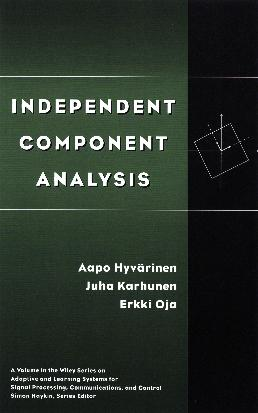
\includegraphics[height=\textheight]{ICABookCover}
\ec

%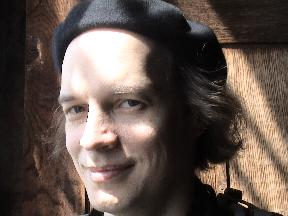
\includegraphics{Aapo}
%\begin{block}{}
%Independent component analysis (ICA) is a statistical and computational technique for revealing hidden factors that underlie sets of random variables, measurements, or signals.
%\end{block}
}

\frame{
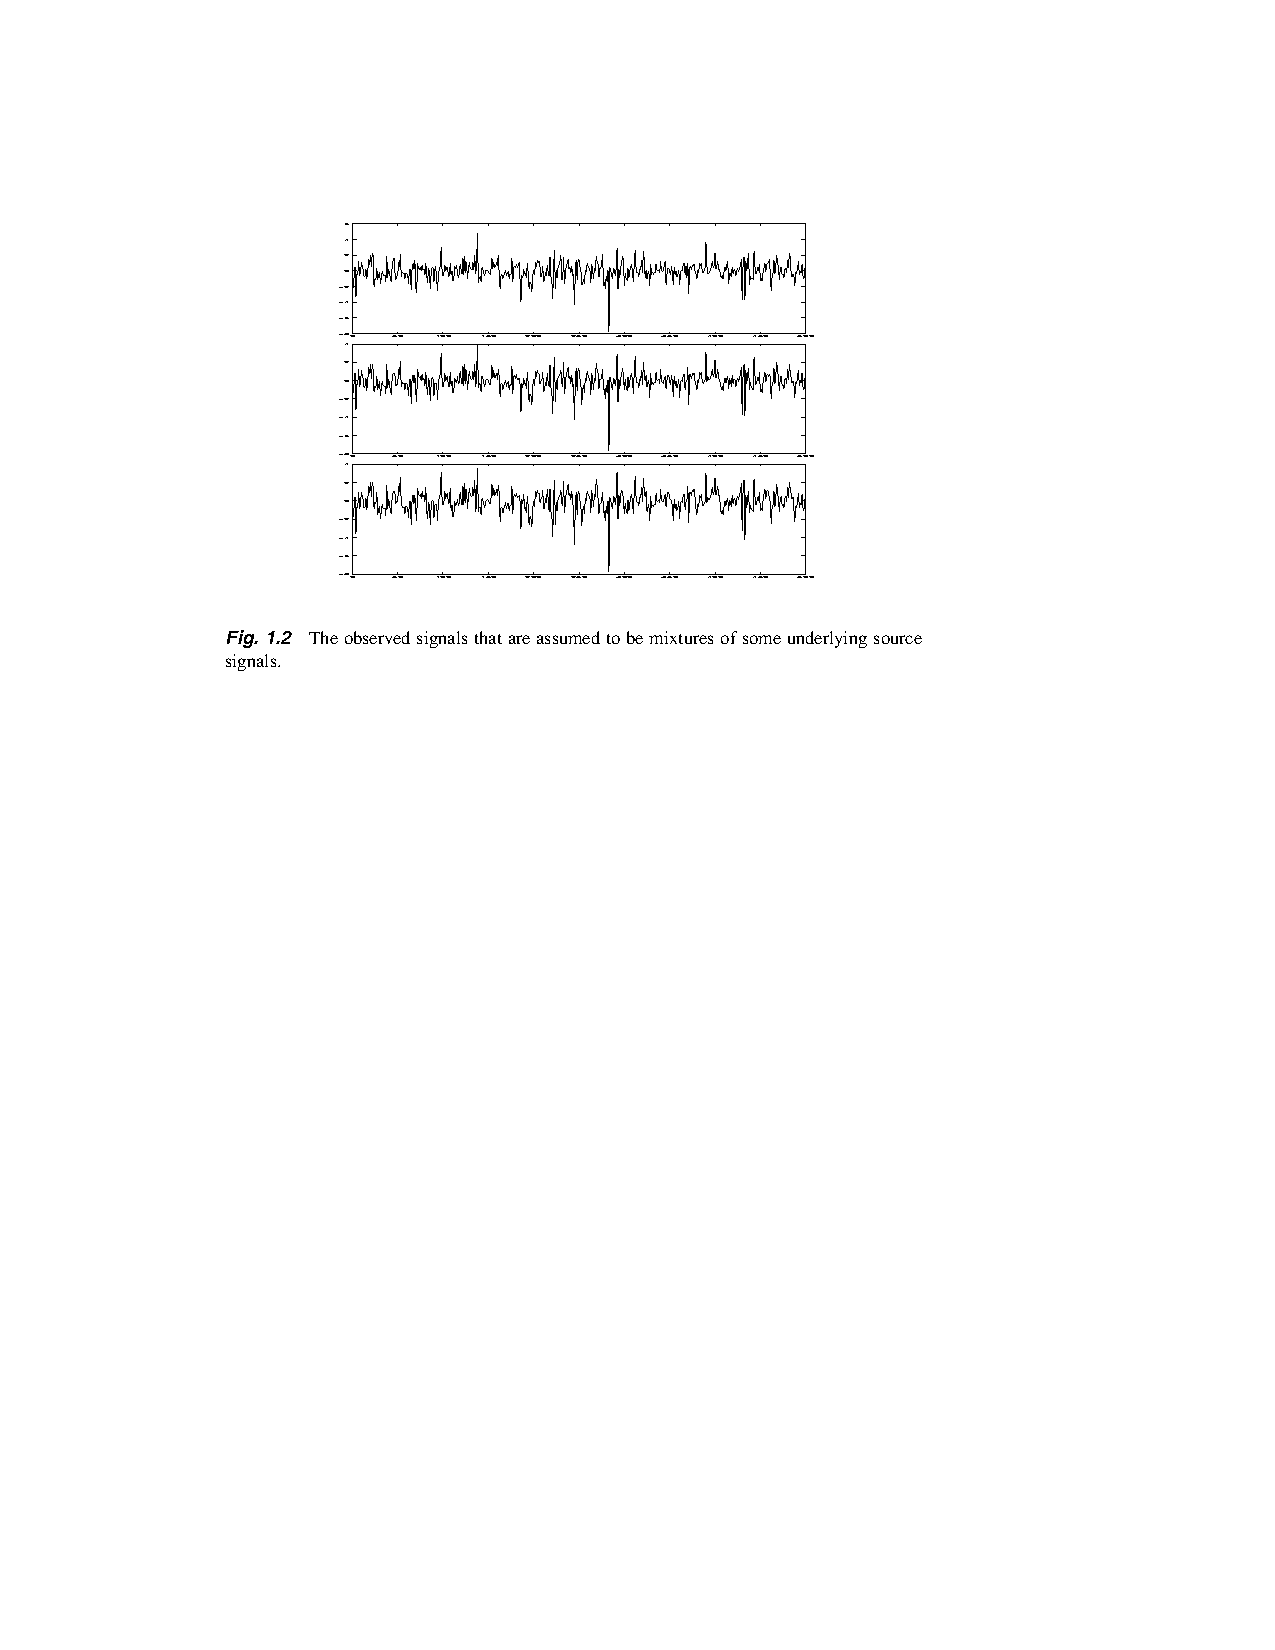
\includegraphics{ICABOOK2001_ObservedSignals}
}

\frame{
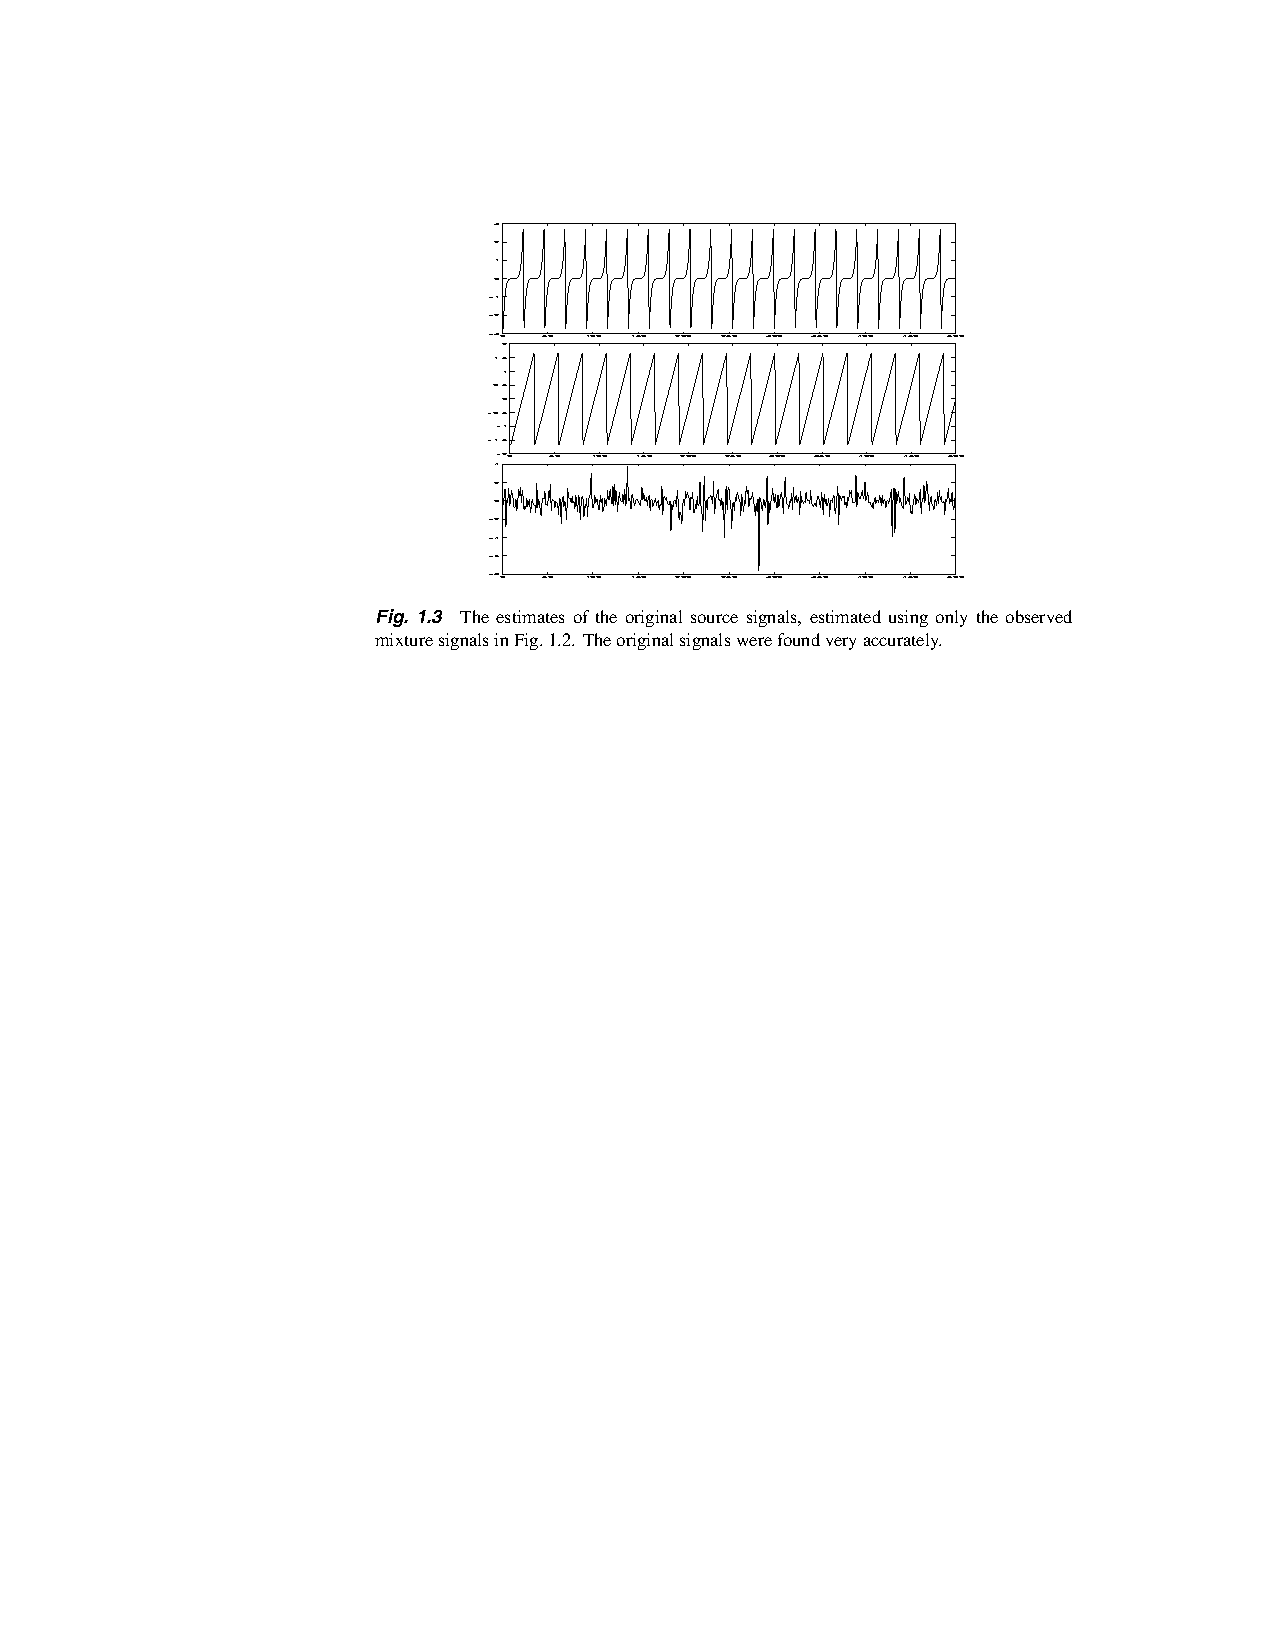
\includegraphics{ICABOOK2001_ReconstructedSignals}
}


\frame{
{
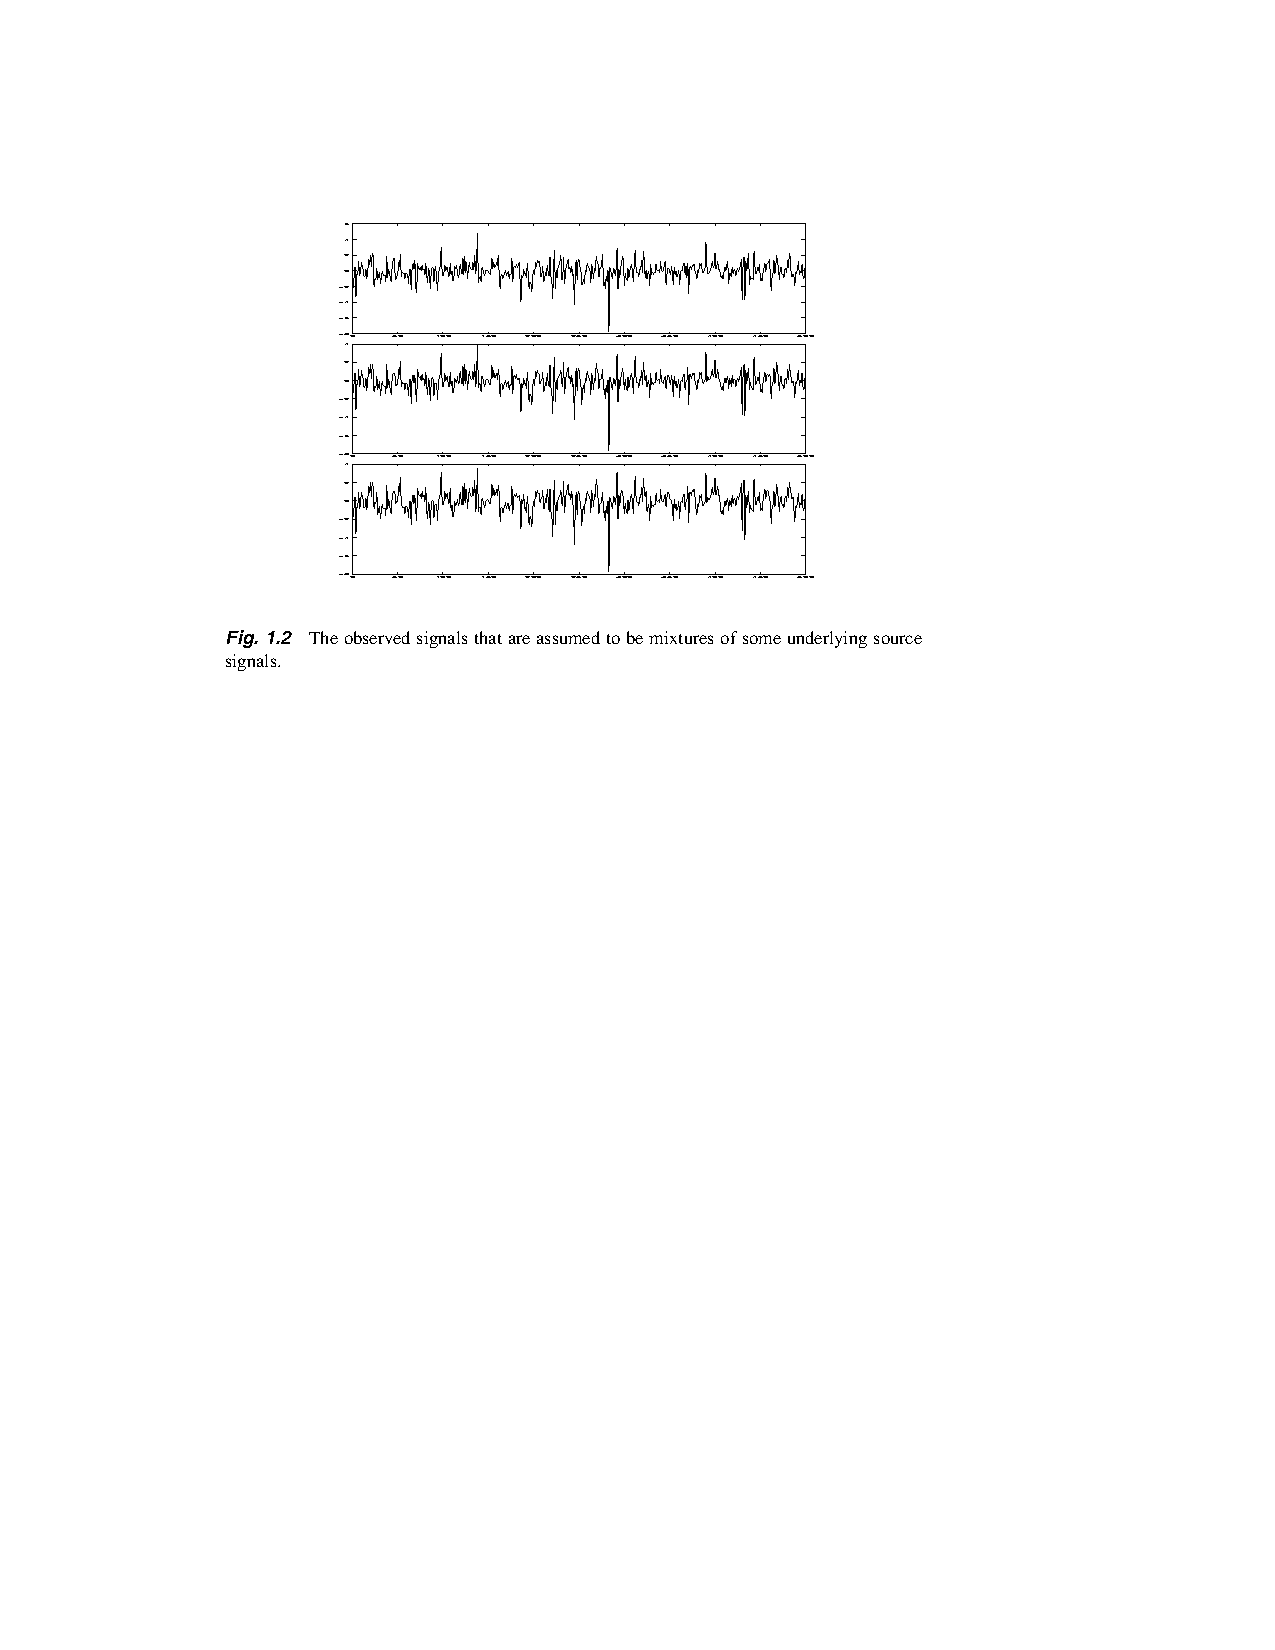
\includegraphics[width=0.3\textwidth]{ICABOOK2001_ObservedSignals}
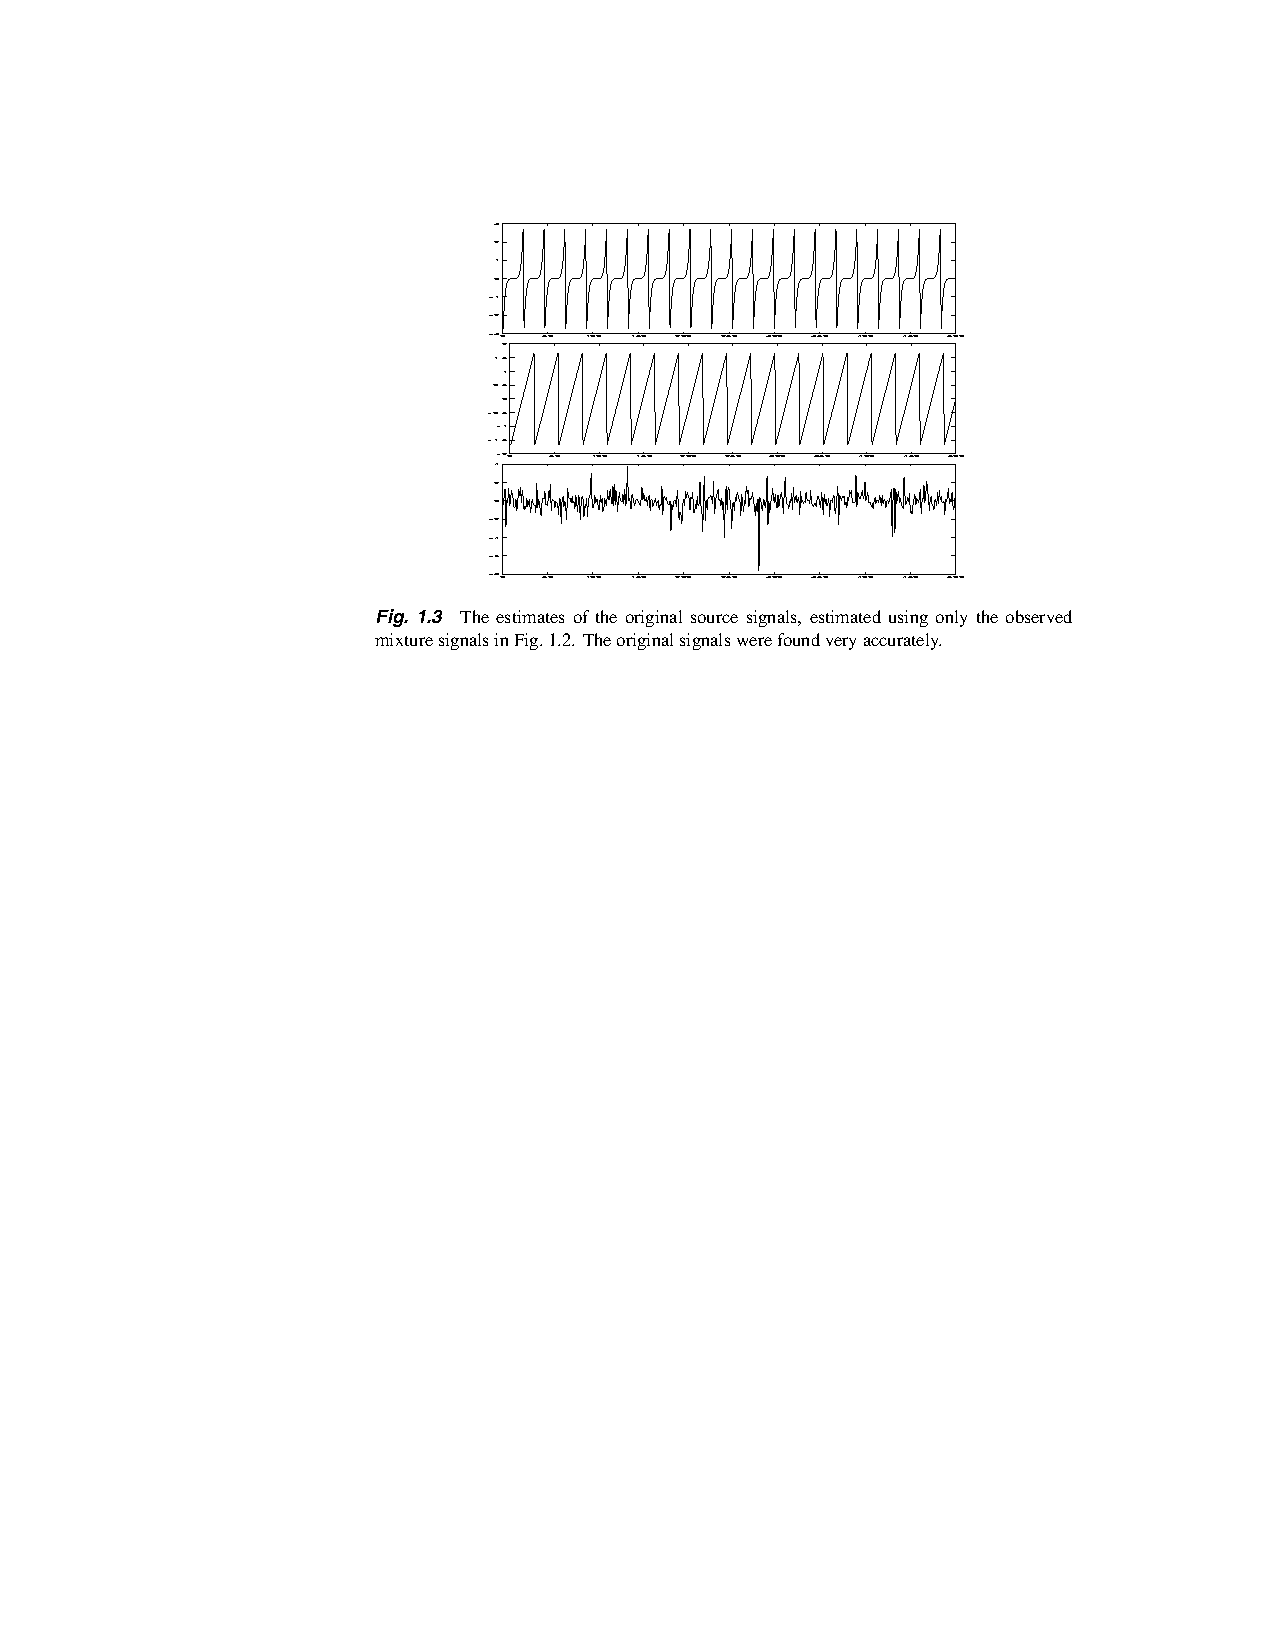
\includegraphics[width=0.3\textwidth]{ICABOOK2001_ReconstructedSignals}
}
%\vspace*{-0.5in}
\begin{quotation}
\uncover<+->{%
We were able to estimate the original source signals, using an algorithm that used the information on the \alert{independence only}. [$\dots$]
}
\uncover<+->{This leads us to the following definition of ICA [$\dots$]}
\uncover<+->{Given a set of observations of random variables
$(x_1(t),x_2(t),\dots,x_d(t))$, 
where $t$ is the time or sample index, 
assume that they are generated as a linear mixture of \alert{independent components}:
\[
\begin{pmatrix}
x_1(t)\\x_2(t)\\ \vdots \\ x_d(t)
\end{pmatrix} = A
\begin{pmatrix}
s_1(t)\\s_2(t)\\ \vdots \\ s_d(t)
\end{pmatrix}\,,
\]
where $A$ is some unknown matrix.}
\end{quotation}
}



\frame{
\bc
\LARGE Good?
\ec
}

\frame{
\frametitle{Independence?}
\bc
\vspace*{-0.45in}
\mbox{}\hspace*{0.5\textwidth}
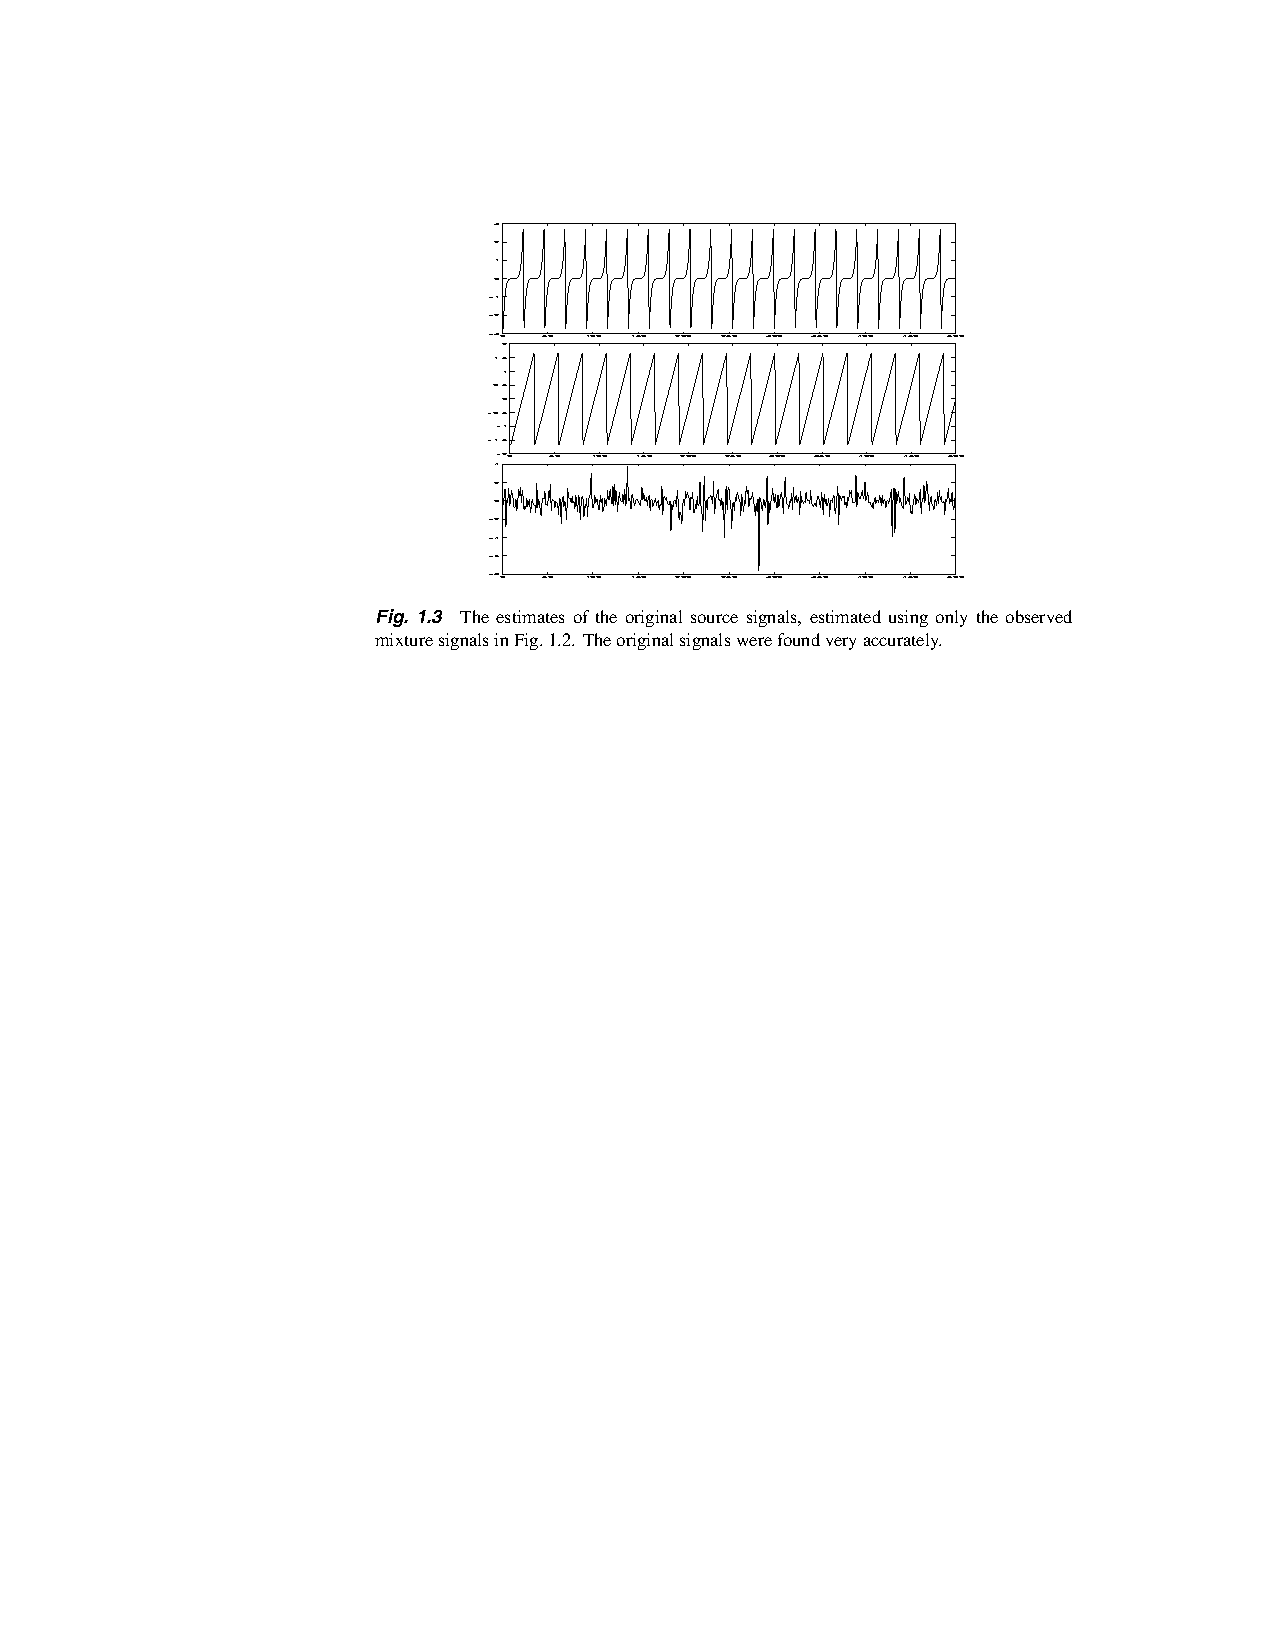
\includegraphics[width=0.45\textwidth]{ICABOOK2001_ReconstructedSignals}
\ec
\bi
\item Is $s_1(t)$ independent of $s_2(t)$? \uncover<+->{Sure!}
\item Any two numbers are independent of each other! 
\uncover<+->{All deterministic signal sources are fine then?}
\item Should we be worried about temporal dependencies? \uncover<+->{No?}
\uncover<+->{What if $s_1(t) = s_1(t+1) = \dots$? }
\item Can we redefine ICA in a more meaningful way?
\item \alert{Let's go beyond statistics!}
\ei
}

\frame{
\frametitle{How to go beyond statistical analysis?}
\begin{enumerate}[<+->]
\item Perform a deterministic analysis of the algorithm, reducing the problem to perturbation analysis
\item Perform statistical analysis on the size of perturbations when necessary or desired
\end{enumerate}

\begin{block}<+->{History}
\bi
\item Online learning (adversarial, regret analysis of learning algorithms) \citet{CBLu06:book}
\item Regression analysis: \citet{vito2006learning}
\item Value function estimation in RL: \citet{PiSze1206}
\item ICA: This work
\ei
\end{block}
}

\section{Deterministic ICA}
\begin{frame}{Outline}
\tableofcontents[currentsection,currentsubsection]
\end{frame}

\frame{
\frametitle{Deterministic ICA}
\bi
\item What signals can be separated?
\item Better: To what extent can we separate the mixture of some signals? 
\ei
\uncover<+->{
Let $[T] = \{1,\dots,T\}$.
Sources:  $s:[T] \to [-C,C]^d$.
}

\uncover<+->{
Let $\nu^{(s)}$ be the empirical distribution induced by $s$; for $B\subset [-C,C]^d$,
	\[
	\nu^{(s)}(B)=\tfrac{1}{T}|\{t \in [T]: s(\tau) \in B\}|.
	\]
}
\bi
\item Measure of independence: $D_4(\nu^{(s)},\mu)$, $D_4^{(d,d)}(\nu^{(As,\eps)})$;
\item Measure of Gaussianness: $\kappa(\nu^{(\eps)})$;
\item Measure of Zero-Mean: $N(\nu^{(\eps)})$, $N(\nu^{(s)})$
\ei

}

\if0
\frame{
\frametitle{Deterministic ICA}
\begin{block}<+->{Measure of independence}
%Our independence measure:
	\[
	D_4(\nu_1,\nu_2)	= \sup_{f\in\mathcal{F}} \Big|\int f(s)\nu_1(ds) - \int f(s)\nu_2(ds)\Big|,
	\]
 $\mathcal{F}$: the set of all monomials up to degree $4$; \\
  When $\nu$ is a measure of $p+q$ variables (i.e., $X\in \mathbb{R}^{p+q}$) 
  \[D_4(\nu) = \inf_{\mu\in \Pi} D_4(\mu,\nu); \quad D_4^{(p,q)} (\nu)= \inf_{\mu_1,\mu_2} D_4(\mu_1\otimes \mu_2,\nu).
  \]
\end{block}
\begin{block}<+->{Measure of Gaussianness}
	\begin{align*}
		\kappa^2(\mu) = & \max_{1\le i,j\le d} \sum_{k,l} 
		\big\{ 
		M_{i,j,k,l}(\mu)  - (M_{i,j}(\mu) M_{k,l}(\mu)+  M_{i,k}(\mu) M_{j,l}(\mu) \\
		& \quad  + M_{i,l}(\mu) M_{j,k}(\mu))
		\big\}^2,
	\end{align*}
   where $M_{a,\dots,z}(\mu) = \int y_a \dots y_z \mu(dy)$.
\end{block}
\begin{block}<+->{Measure of Zero Mean}
	\[
 	N(\nu) = ||\int x \nu(dx) ||_F
	\]
\end{block}
\begin{block}<+->{Measure of Accuracy}
	\[ d(\hat{A},A) = \inf_{\substack{\pi \in \mathrm{Perm}([d]) c\in \real^d}} \max_{k} || c_k A_{:\pi(k)} - A_{:k} ||_2\,.\]	
\end{block}
}

\frame{
\frametitle{Goal}
Assuming $x(t) = A s(t) + \eps(t)$, $t=1,\dots, T$;
\\ $\eps(t)$ ``noise''.\\

\medskip

Can we find a method with the following characteristics?

\bi
\setlength{\itemsep}{10pt}
\item[\ds] Universal: No free parameters!
\item[\ds] Efficient:  $\mathrm{poly}(T,d)$ runtime (no dependence on $C$, $A$, $\dots$);
\item[\ds] Robust \& noise-tolerant: $\mathrm{lin}(D_4+1/\sqrt{T})$ accurate in recovering $A$ (with i.i.d. observation noise)?
\ei

\uncover<+->{
Accuracy measure:
\[
d(\hat{A},A) = \inf_{
	 \substack{\pi \in \mathrm{Perm}([d])\\
	 c\in \R^d}} \max_{k} 
	|| c_k A_{:\pi(k)} - A_{:k} ||_2\,.
\]
}
}

\subsection{Has not this been done previously?}
\begin{frame}{Outline}
\tableofcontents[currentsection,currentsubsection]
\end{frame}

\frame{ 
\frametitle{Previous works with theoretical guarantees} 

\onslide<+->
\citet{SaTsy04,CheBi06} and others: 
\bi
\item No noise
\item Semi-parametrics, ``average derivative estimation'';
\item Asymptotics: $\sqrt{n}$ consistency and efficiency;
\item Why estimate something that is then thrown away? (Also: We'll need conditions on these$\dots$)
\ei
\medskip

\onslide<+->
FastICA by \citet{hyvarinen1999fast}:
\bi
\item Perhaps the most popular ICA algorithm.
\item With probability 1, all local optimizers are desired solutions \citep{wei2014study}, given:
	\begin{itemize}
	\item[--]<2-> infinitely many noiseless samples;
	\item[--]<2-> using kurtosis as the scoring function.
	\end{itemize}
\item[-] Weakness: noisy periodic signals;
\ei

\onslide<+->
%\vspace{1cm}
Moment methods: \citep{frieze1996learning,DHsu2012, arora2012provable,goyal2014fourier}.
}

\frame{ \frametitle{Moment methods}
\bi
\item \citet{frieze1996learning}: 
\bi
\item[-] No noise allowed (also: minor gap fixed by \citet{arora2012provable});
\ei
\item \citet{DHsu2012} (``HKICA''):
\bi
\item[-] No theoretical guarantee stated;
\item[-] If we do the analysis, accuracy will depend on $\gamma_A$; an uncontrolled parameter (see later).
\ei
\item \citet{arora2012provable}:
\bi
\item[-] Free parameter ``$\beta$'', whose choice depends on $||A_{:i}||_2$, while $x\in \{-1,+1\}^d$.
\item[-] Choose either the scale of sources or the scale of the columns of $A$, not both!
\ei
\item Fourier PCA \citep{goyal2014fourier} (FPCA):
\bi
\item[-] Free parameter: Same problem as with \citet{arora2012provable}'s approach.
\ei
%\\
%\quad - If you assume that both the mixing matrix and the sources are bounded with a known bound, 
%the parameter can be chosen.
%\\
\ei

\uncover<+->{\centering \alert{Why care about a free parameters?}}
\uncover<+->{\centering $\dots$ \textcolor{blue}{unsupervised} learning}
%This is unsupervised learning!\\
%Cross-validation is messy at best.
%\end{block}
}
\fi

\frame{ \frametitle{Result}
There exists a randomized algorithm such that 
for any $A\in \real^{d\times d}$, and $x, s, \eps: [T] \rightarrow \real^d$ satisfying $x(t) = As(t)+\eps(t)$,
the algorithm returns $\hat{A}$ such that:
\bi 
\item The computational complexity is $O(d^3 T)$;
\item With high probability, 
\begin{align*}
d(\hat{A}, A) \le & 
\inf_{\mu\in \Pi_0} \mathcal{C}(\mu) \min\Big(D_4(\nu^{(s)},\mu)+ \kappa(\nu^{(\eps)}) + D_4^{(d,d)}(\nu^{(As,\eps)}) \\
& \quad +N(\nu^{(\eps)}) + N( \nu^{(s)}), \Theta(\mu) \Big),
\end{align*}
\item Here,$\mathcal{C}(\mu)$ and $\Theta(\mu)$ are problem dependent, polynomial in the parameters.
\ei
}


\section{Conclusions}
\begin{frame}{Outline}
\tableofcontents[currentsection]
\end{frame}

\frame{\frametitle{Conclusions and Open Questions}

\bi
\item[\ds] Independent Component Analysis without probabilities! 
\item[\ds] Deterministic analysis: Cleaner, more general, should do it more often! Limits?
\item[\ds] New method: DICA. Universal, strong guarantees.
\ei

\vspace{1.5cm}
\uncover<+->{
\centering 
{\LARGE \textcolor{blue}{Questions?}}
}
}

\frame{ \frametitle{References}
\tiny
\bibliographystyle{abbrvnat}
\bibliography{DICA}
}
\end{document}
